\chapter{Theorie}
\label{cha:Theorie}
Nun werden die theoretischen Grundlagen zu diesem Versuch motiviert. Bei Wasserstoff als einfachstes Element lassen sich klassisch Absorptionslinien oder Emissionslinien,
welche kein dispersives Spektrum aufweisen nicht erklären. Wird das Problem nun aber Quantenmechanisch betrachtet wurde erkannt, dass sich das Elektron um den Kern herum auf sehr genau 
definierten Energieniveaus befindet. Diese Enegrieniveaus können durch die jeweiligen relevanten Quantenzahlen beschrieben werden. Dazu gehören die Hauptquantenzahl $n$,
die Bahndrehimpulsquantenzahl $l$ und die magnetische Quantenzahl $m$. $n$ darf nur Werte in den natürlchen Zahlen einnehmen. $l$ is auf alle natürlchen Zahlen, die kleiner als $n$
sind beschränkt und $m$ kann Werte von $-l < m < l$ annehmen. Diese Überlegung funktioniert nur sehr gut solange wir ein Zwei-Körper-Problem betrachten. Aber Näherungsweise gilt dieses 
Modell auch für Alkali-Metalle aufgrund des einzelnen Valenzelektrons.

\section{Spin-Bahn-Kopplung}
\label{sec:soc}
Wird nun das Elektron in seinem Ruhesystem betrachtet, sodass das Proton um das Elektron \enquote{rotiert}, besagen die Maxwellgleichungen, dass die bewegte Ladung ein Magnetfeld 
induziert. Der Spin des Elektrons koppelt an das induzierte Magnetfeld, weshalb sich die Energieniveaus aufspalten. Der Drehimpuls $J = L + S$ spaltet sich dabei 
in ganzzahlige Werte von $|L-S|$ bis $L+S$ auf. Aufgrund des einzelnen Valenzelektrons ist der Grundzustand von \ce{^{85}Rb} und \ce{^{87}Rb} ein s-Orbital. Daher haben beiden Isotope 
$J = \frac{1}{2}$.

\section{Hyperfeinstruktur}
\label{sec:hfs}
Genau wie das magnetische Moment des Elektrons kann auch das magnetische Moment des Kern an Magnetfelder koppeln und für eine Spaltung der Energieniveaus sorgen. Diese Aufspaltung wird 
Hyperfeinstruktur genannt. Diese lässt sich durch die zugehörige Quantenzahl $F$ beschreiben. Es werden Werte von $|J-I|$ bis $J+I$ angenommen. Mit den Kernspins $I$ von 
\ce{^{85}Rb} mit $I = \frac{5}{2}$ und \ce{^{87}Rb} mit $I = \frac{3}{2}$ erhalten wir jeweils eine Aufspaltung in zwei Mögliche Werte für $F$.

\section{Zeemann-Effekt}
\label{sec:zeemann}
Eine weitere Aufspaltung ist durch den Zeemann Effekt gegeben. Hierbei handelt es sich um eine externe Aufspaltung durch Magnetfelder. Die Quantenzahl F spaltet sich nun weiter auf.
Erneut koppelt das magnetische Moment des Kerns an das Magnetfeld. Dies sorgt für eine Aufspaltung von $-F < m_F < F$. Es entstehen $2F+1$ Energieniveaus. Die Energiekorrektur 
der einzelnen Niveaus lautet 
\begin{equation}
              \label{eqn:dEz}
              \Delta E_z = g_F\mu_BB \,.
\end{equation}

In dieser Gleichung ist $\mu_B$ das Bohrsche Magneton, $B$ das Magnetfeld und $g_F$ der Land\'{e}-Faktor. Dieser ist gegeben mit 
\begin{equation}
              \label{eqn:g_F}
              g_F = g_J \frac{F(F+1)+J(J+1)-I(I+1)}{2F(F+1)}\,,
\end{equation}
und 
\begin{equation}
              \label{eqn:g_j}
              g_J = 1 + \frac{J(J+1)+S(S+1)-L(L+1)}{2J(J+1)}\,.
\end{equation}

Eine Nivauschema wird in Abbildung \ref{fig:energieschema} dargestellt.

\begin{figure}
              \centering
              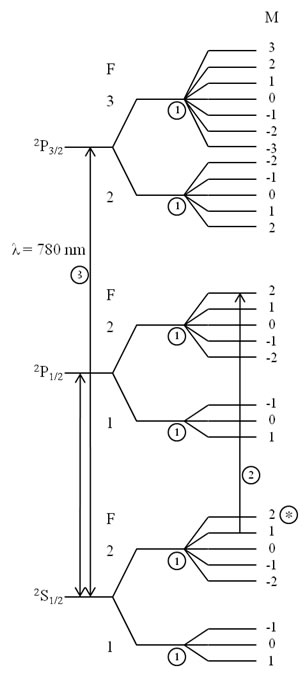
\includegraphics[height = \textheight]{content/v21_bilder/zeeman_splitting.jpg}
              \caption{Niveauaufspaltung in Rubidium.}
              \label{fig:energieschema}
\end{figure}

\section{Optisches Pumpen}
\label{sec:pumpen}
Mit diesem Modell der Niveauspaltung kann das Wasserstoff Atom und ähnliche Moleküle, also Alkalimetalle, beschrieben werden. Bei einem einzelnem Atom isolierten Atom wird natürlich 
erwartet, dass sich dieses in einem stabilen Zustand der niedrigsten Energie aufhält. In einem Vielteilchen-System, wie beispielsweise ein Gas, verhält sich die Physik des 
Valenzelektrons etwas anders. In einem solchen System müssen Wechselwirkungen der Teilchen miteinander und der Umwelt betrachtet werden. Allem voran ist die endliche Temperatur 
und der Druck ausschlaggebend für kleine Anregungen im System. Die Gas-Moleküle bewegen sich dauerhaft und kolliedieren miteinander. Eine Kollision kann die kinetische Energie umwandeln 
und das Valenzelektron in einen angeregten Zustand anheben. Aus statistischer Betrachtung folgt, dass sich die einzelnen Energieniveaus nach einer Bolzmann-Verteilung füllen. 

Um nun Elektronen aus dem $^2S_{1/2}$ Grundzustand in einen anderen Zustand anzuheben muss exakt die Energiedifferenz über ein Photon bereitgestellt werden. Licht, welches 
einen Übergang von $^2S_{1/2}$ nach $^2P_{1/2}$ ermöglicht, wird $D_1$-Licht genannt. Die Auswahlregel erlaubt lediglich $\Delta M = \pm 1$ für rechts-/links zirkularpolarisiertes Licht und 
$\Delta M = 0$ für linearpolarisiertes Licht. Die Übergänge für rechts zirkularpolarisiertes Licht werden $\sigma^+$, die anderen $\sigma^-$ genannt. Optisches Pumpen verwendet nun genau,
dass durch zirkular polarisiertes Licht einer der Grundzustände angeregt werden kann, ohne die anderen zu beeinflussen. Daher wird nun ein Vielteilchensystem an Alkalimetallen mit 
rechts zirkularpolarisiertem Licht bestrahlt. Alle Elektronen im $\Delta M = 1$ Zustand werden dann vom $S$ ins $P$ Niveau gehoben. Dieser angeregte Zustand ist lediglich Metastabil.
Die Heisenbergsche Unschärfe-Relation für Energie und Zeit besagt nun, dass in einem sehr kleinen Zeitintervall die Energeiunschärfe sehr groß sein kann. Aufgrund dieser Quantenfluktuation 
wird das Elektron im $P$ Zustand dazu angeregt ein Photon zu emittieren und sich in seinen Grundzustand zu begeben. Dabei ist es gleichwhrscheinlich in welchen Zustand es übergeht.
Durch konstante Bestrahlung mit rechts zirkularpolarisiertem Licht werden die ELektronen so also in den anderen Grundzustand \enquote{gepumpt}. Nach unendlich langer Zeit befinden sich 
alle Elektronen im $\Delta M = -1$ Zustand. In diesem Zustand kann das rechts zirkularpolarisiertem Licht nicht mehr mit dem Gas koppeln. Dieser Zustand wird Besetzungsinversion genannt.
Neben dem natürlichen Prozess, häufig spontane Emission gennant, kann auch eine stimulierte Emission durch ein äußeres hochfrequentes Magnetfeld stattfinden. Die Wahrscheinlichkeit
für eine stimulierte Emission ist proportional zu $f$. Da die Wahrscheinlichkeit für spontane Emission lediglich proportional zu $f^3$ ist, kann dieser Prozess vernachlässigt werden.

\section{Durch Zeemann-Aufspaltung zum Kernspin}
\label{sec:landee}

Wird das Rubidium-Gemisch in seinem Grundzustand optisch gepumpt, so steigt die Transparenz des Gases zunächst stark an. Zu Beginn ist es quasi undurchlässig für das verwendete 
$D_1$-Licht, da jedes Photon absorbiert werden kann. Nach genügend andauernder Bestrahlung wird das Gas, in welchem nun eine Besetzungsinversion vorliegt, transparent für das Licht. 
Dieser Prozess wird durch die Abbildung \ref{fig:transparenz} deutlich.

\begin{figure}
              \centering
              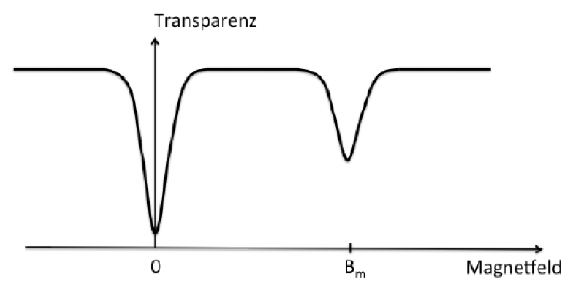
\includegraphics[width = \textwidth]{content/v21_bilder/transparenz.PNG}
              \caption{Änderung der Transparenz des Gases durch optisches Pumpen und resonante Anregung eines RF-Feldes. \cite{v21}}
              \label{fig:transparenz}
\end{figure}

Wie bereits diskutiert führt eine äußeres Magnetfeld zu einer Zeemann-Spaltung der Energieniveaus abhängig von der Stärke des Magnetfeldes gemäß Formel \eqref{eqn:dEz}. 
Wenn die Zeemann-Aufspaltung nun genausogroß wird, wie die Energie des $D_1$-Lichts, dann kann durch stimulierte Emission ein Bruch der Besetzungsinversion stattfinden. 
Dies kennzeichnet sich durch einen kleineren Dip im Transparenz-Plot \ref{fig:transparenz}. Dies lässt sich als Formel ausdrücken durch 
\begin{equation}
              \label{eqn:g_formel}
              hf = g_F\mu_BB \,.
\end{equation}
In dieser Gleichung ist $h$ das planksche Wirkungsquantum und $f$ die Frequenz des Lichtes. Anhand von Gleichung \eqref{eqn:g_formel} kann der Land\'{e}-Faktor bestimmt werden, 
indem an der stelle des resonanten RF-Felds, welches in Abbildung \ref{fig:transparenz} durch $B_m$ gekennzeichnet ist, die Gleichung gelößt wird und nach $g_F$ umgestellt wird.
Aus $g_F$ kann dann über Gleichung \eqref{eqn:g_F} der Kernspin berechnet werden.
Bei einem Gemisch aus unterschiedlichen Isotopen treten mehrere Peaks in der Transparenz auf, da der Kernspin und andere Größen anders sind. 